\chapter{The State-of-the-Art in User Steering Action Data Analysis}
\label{chap3}

As discussed in the introduction (Chap. \ref{chap_intro}), steering actions are the individual interactions that the user performs while they are steering a CSE application running on a large-scale machine.
Several surveys, both old~\cite{MulderSurvey,Xian2008Computational} and recent ones~ \cite{Ayachit2016Performance, Bauer2016In}, have analyzed multiple approaches to support user steering and others, also recent~\cite{deelman_future_2017,Mattoso2015Dynamic,F.daSilva2017characterization,Atkinson2017Scientific,Netto2018HPC}, further highlight the importance of dynamic steering in workflows.
Particularly, \citet{Mattoso2015Dynamic}
  analyzed approaches implemented within WMSs analyzing their steering and provenance data management support.
In this chapter, we extend the analyses done by these surveys by examining several approaches, within a WMS or not, concerning how they support steering (online analysis and adaptation) and, more importantly, their support for allowing for tracking steering actions.
\crossref{V7: adicionar as figuras da revisao bibliografica}
A search on Google Scholar using keywords related to the content of this thesis returned about 450 papers, among more than 300 have been published in the past few years as shown in Figure \ref{fig:chap3_timeline}.
Among these papers, we investigate in detail over 60 papers related to this work, as we present in the next sections. Among these papers, we identified 54 approaches, where 7 are based on a WMS and 47 are not (Fig. \ref{fig:chap3-wms-vs-nowms}). To the best of our knowledge, this is the first state-of-the-art analysis in the context of user steering in large-scale workflows that examines approaches both within and without WMSs.
We begin this chapter by investigating the types of steering actions supported in the state-of-the-art. We could identify two main types: online data analysis and online data adaptation. These two can be further classified as shown in Figure \ref{fig:chap3_taxonomy}, and detailed as follows.


\begin{figure}
\centering
\begin{subfigure}{.6\textwidth}
  \centering
  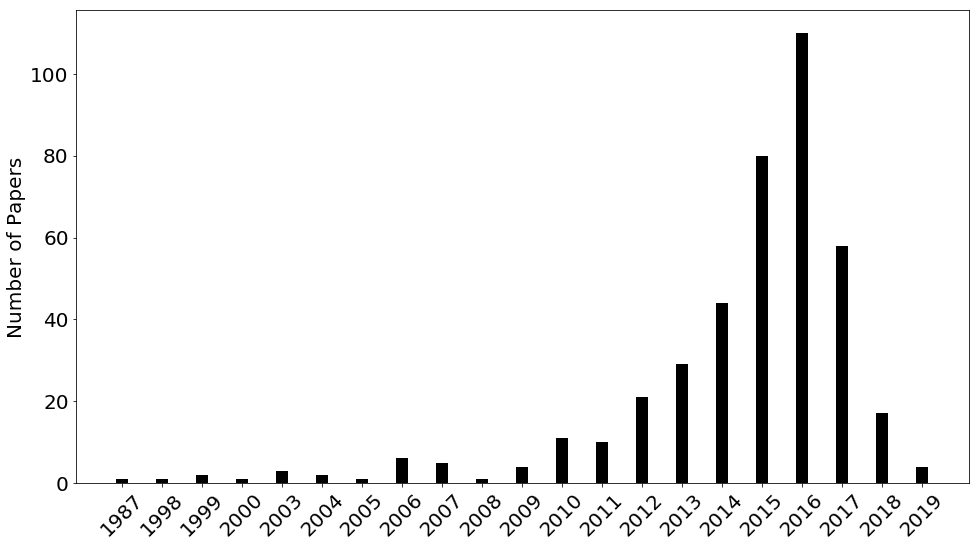
\includegraphics[width=1.0\linewidth]{img/timeline.png}
  \caption{Amount of papers analyzed in our search in the past years.}
  \label{fig:chap3_timeline}
\end{subfigure}%
\begin{subfigure}{.1\textwidth}
  % \centering
  % 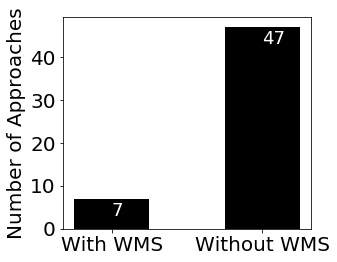
\includegraphics[width=1.0\linewidth]{img/chap3-wms-vs-nowms.png}
  % \caption{Number of approaches that use or not WMSs.}
  % \label{fig:chap3-wms-vs-nowms}
\end{subfigure}
\begin{subfigure}{.3\textwidth}
  \centering
  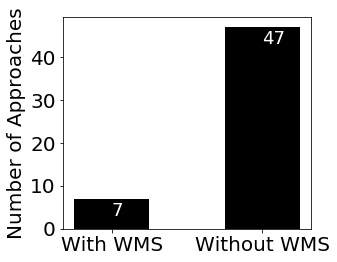
\includegraphics[width=1.0\linewidth]{img/chap3-wms-vs-nowms.png}
  \caption{Number of approaches that use or not WMSs.}
  \label{fig:chap3-wms-vs-nowms}
\end{subfigure}
%\caption{}
% \label{fig:chap3-wms-vs-nowms}
\end{figure}


%
% \begin{figure}[H]
%     \centering
%     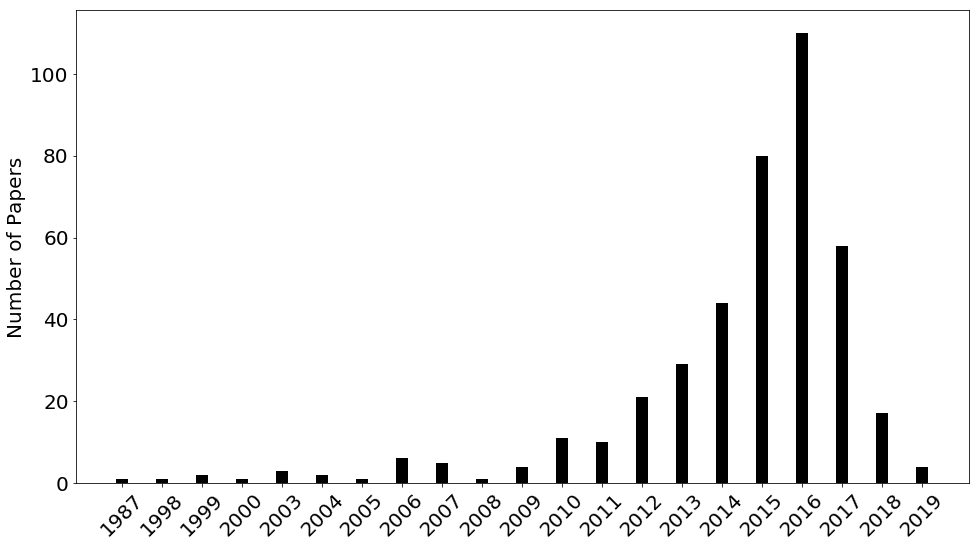
\includegraphics[width=\textwidth,keepaspectratio]{img/timeline.png}
%     \caption{Amount of papers analyzed in our search in the past years.}
%     \label{fig:chap3_timeline}
% \end{figure}
%
% \begin{figure}[H]
%     \centering
%     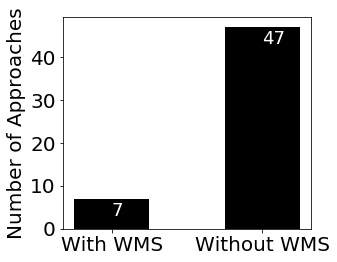
\includegraphics[width=\textwidth,keepaspectratio]{img/chap3-wms-vs-nowms.png}
%     \caption{Number of approaches that use or not WMSs}
%     \label{fig:chap3-wms-vs-nowms}
% \end{figure}


\begin{figure}[H]
    \centering
    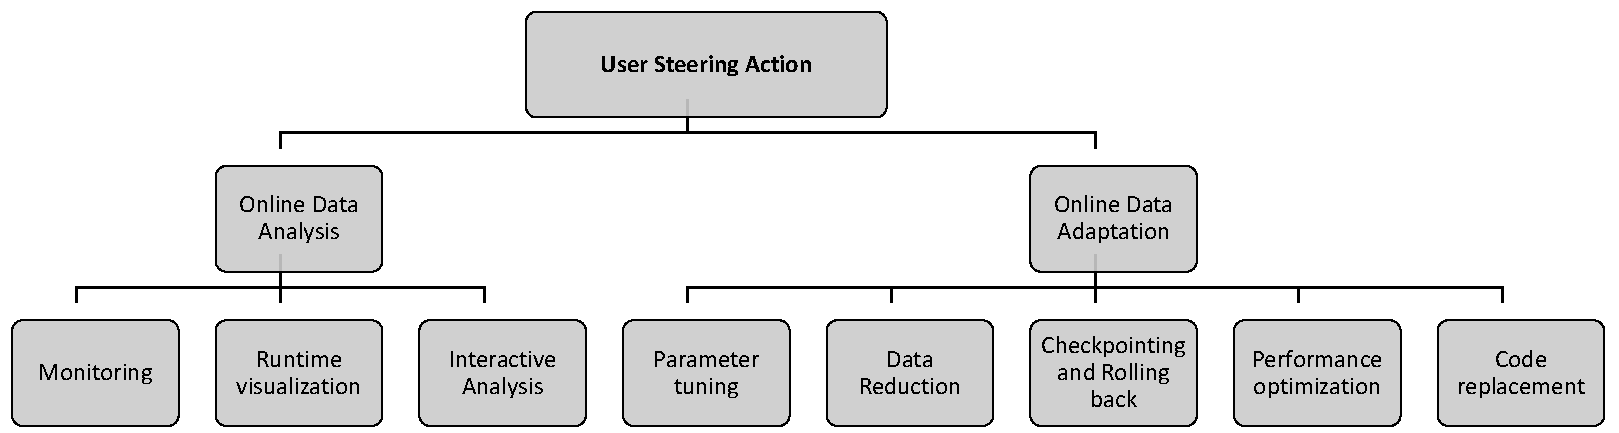
\includegraphics[width=\textwidth,keepaspectratio]{img/taxonomy-chap3.pdf}
    \caption{A taxonomy for user steering actions.}
    \label{fig:chap3_taxonomy}
\end{figure}


In case of online data analysis, we can further identify the following actions:

 \begin{itemize}
 \setlength\itemsep{-2mm}

    \item[-] \textit{Monitoring} --- a predefined data analysis plotted as charts in a dashboard or tables, whose results are refreshed in predefined time intervals. Usually, users follow the monitoring results passively, with less interaction. Depending on the monitoring results, users can interact with the workflow;

    \item[-] \textit{Runtime visualization} --- a data analysis where there are scientific data visualization techniques involved, often combined with computer graphics tools and HPC techniques that allow for visualizing the large scientific data at runtime;

    \item[-] \textit{Interactive analysis} --- a data analysis that allows users to perform \textit{ad-hoc} exploratory analysis over the workflow data. This is different from monitoring in the sense that the former requires predefined specification of what is going to be analyzed, whereas the latter enables more interactive queries as the user can change what is being analyzed as they analyze the partial results.

 \end{itemize}

In case of online data adaptation, we can further identify the following actions:

 \begin{itemize}
\setlength\itemsep{-2mm}

    \item[-] \textit{Parameter tuning} --- dynamic changes of parameter values of data transformations in a dataflow, such as fine-tune simulation parameters of a computational model,
    change loop-stop conditions;

    \item[-] \textit{Data reduction} --- dynamic removal of input data that the user decided that should not be processed, such as pruning possible solutions of a large solution space being explored in parallel that are no longer
interesting (\eg{} the solutions are unfeasible or not optimal).

    \item[-] \textit{Checkpointing and rolling back} --- specification of certain points, during workflow execution, that the user marked ``safe'' or had the expected results. If a failure happens, e.g., program crash, function not con-verging as excepted, or even failure caused by external factors, such as hardware failure, the user would be able to request a rollback to one of the check-pointed states. This facilitates ``what-if'' exploration
    \cite{Bourhis2016Analyzing}.

    \item[-] \textit{Performance optimization} --- dynamic tunes in the application data or computing resources at runtime aiming at improving performance or saving resources, \eg{} change the load of
    processor units that are overloaded.

    \item[-] \textit{Code replacement}  --- modification of parts of a running code (also
known as ``live programming'').


 \end{itemize}

 Then, in the following sections, we analyze the approaches available in the literature, in the context of user steering support.




\section{Approaches for Online Analysis, Adaptation, and User Steering Action Data Management}

Table \ref{tab:comparative_tables_systems} summarizes the approaches on  online data analysis support, which online adaptations they support, and whether or not they allow for tracking user steering actions.
We particularly investigate, for example, if they manage steering action data or
any other data for data analysis or reproducibility.

\begin{longtable}
{ 
 M{.17\textwidth}||
 M{.25\textwidth}|
 M{.25\textwidth}|
 M{.20\textwidth}
}
\caption{Comparison  of  approaches for user steering support.}
\label{tab:comparative_tables_systems}\\
 \hline
 \hline
 \hline
 \hline
 \rowcolor{TableHeaderColor}

  \textbf{Approach} &
  \textbf{Online Data Analysis} &
  \textbf{Online Data Adaptation} &
  \textbf{Tracking Steering Actions}
 \\
 \hline
 \hline
 \hline
 \endhead


\textbf{DfAnalyzer}
\cite{Silva2017Raw,Camata2018In,silva_dfanalyzer:_2018}
 &
Monitoring, interactive data analyses, runtime visualization
 &
\redx{}
 &
\redx{}
\\
\hline

\textbf{VASE} \cite{Jablonowski1993VASE:}
&
Monitoring
&
Parameter tuning, Code replacement
&
\redx{}
\\
\hline




\textbf{SCIRun}  \cite{Parker1995SCIRun:}
&
Monitoring and runtime visualization
&
Parameter tuning
&
\redx{}
\\
\hline


\textbf{CSE} \cite{Liere1996Computational,Liere1997Computational,Wijk1994Environment}
&
Monitoring and runtime visualization
&
Parameter tuning
&
\redx{}
 \\
 \hline

\textbf{Progress and Magellan} \cite{Vetter1999Techniques}
&
Monitoring and runtime visualization
&
Parameter tuning
&
\redx{}
 \\
 \hline


\textbf{CUMULVS} \cite{Kohl2006Cumulvs:}
&
Monitoring and runtime visualization
&
Parameter tuning, Check-pointing and Rolling-back
&
\redx{}
\\
\hline

\textbf{VIPER}  \cite{Rathmayer1997tool}
&
Monitoring and runtime visualization
&
Parameter tuning
&
\redx{}
\\
\hline

\textbf{MOSS} \cite{Eisenhauer1998Object-based}
&
Monitoring
&
Parameter tuning, Data reduction
&
\redx{}
\\
\hline

\textbf{gViz} \cite{Wood2003gViz}
&
Monitoring and runtime visualization
&
Parameter tuning
&
\redx{}
\\
\hline

\textbf{DISCOVER} \cite{Mann2001DISCOVER:}
&
Monitoring
&
Parameter tuning
&
\redx{}
\\
\hline

\textbf{MoSt} \cite{Glasner2001Monitoring}
&
Monitoring
&
Parameter tuning and performance
optimization
&
\redx{}
\\
\hline



\textbf{GRASPARC} \cite{Brodlie1993GRASPARC:}
&
Monitoring
&
 Parameter tuning, Check-pointing and Rolling back
&
History Tree for maintaining the track of the simulation after a steering action, which is used to go back to a safe state.
\\
\hline

\textbf{ParaView Catalyst Live} \cite{Ayachit2015ParaView,Bauer2016In}
&
Monitoring and runtime visualization
&
Parameter tuning
&
\redx{}
\\
\hline



\textbf{PathFinder}
 \cite{Reed1996Next}
&
Monitoring
&
Parameter tuning and performance optimization
&
\redx{}
\\
\hline


\textbf{Extempore} \cite{Swift2015Live}
&
Runtime visualization
&
 Code replacement
 &
 \redx{}
\\
\hline


\textbf{Cactus} \cite{Goodale2003Cactus}
&
Monitoring and runtime visualization
&
Parameter tuning, Data reduction
&
\redx{}
\\
\hline


\textbf{EPSN} \cite{Esnard2006Steering}
&
Runtime visualization
&
Parameter tuning
&
\redx{}
\\
\hline


\textbf{pV3} \cite{Haimes1996Concurrent}
&
Runtime visualization
&
Parameter tuning
&
\redx{}
\\
\hline


\textbf{RealityGrid} \cite{Pickles2005practical}
&
Monitoring and runtime visualization
&
Parameter tuning with Check-pointing and Rolling back
 &
 \redx{}
\\
\hline


\textbf{EPIC} \cite{Kress2016Visualization}
&
Monitoring and runtime visualization
&
Parameter tuning
&
\redx{}
\\
\hline


\textbf{CS\_Lite}  \cite{Figueira2004CS_LITE:}
&
 \redx{}
 &
 Parameter tuning
 &
 \redx{}
\\
\hline


\textbf{I-WAY} \cite{Parashar2005Grid}
&
\redx{}
&
Parameter tuning
&
\redx{}
\\
\hline


\textbf{Falcon} \cite{Gu1995Falcon:}
&
Interactive analysis
&
Parameter tuning
&
\redx{}
\\
\hline


\textbf{Autopilot} \cite{Ribler1998Autopilot:}
&
Runtime visualization
&
Parameter tuning
&
\redx{}
\\
\hline


\textbf{WBCSim}  \cite{Goel1999WBCSim:,Shu2011Computational,Shu2006WBCSim:}&
Monitoring and interactive analyses
&
Parameter tuning
&
\redx{}
\\
\hline


\textbf{\citet{Yi2014In-situ}}
&
Monitoring and runtime visualization
&
Parameter tuning
&
\redx{}
\\
\hline


\textbf{\citet{Ma2007In-situ}}
&
Runtime visualization
&
Data reduction via down sampling
&
\redx{}
\\
\hline


\textbf{\citet{Han2016Hybrid}}
&
Monitoring
&
Parameter tuning
&
\redx{}
\\
\hline

\textbf{\citet{Matkovic2011Adaptive}}
 &
Monitoring and runtime visualization
&
 Data reduction of parameter space exploration
&
\redx{}
\\
\hline


\textbf{\citet{Butnaru2013Computational}}
&
Monitoring and runtime visualization
&
Data reduction
&
\redx{}
\\
\hline


\textbf{\citet{Knezevic2011Interactive}}
&
Runtime visualization
&
Parameter tuning
&
\redx{}
\\
\hline
\textbf{\citet{Danani2015Computational}}
&
Monitoring and runtime visualization
&
Parameter tuning
&
\redx{}
\\
\hline

%%%%%%%%%%%%%%%%%%%% BEGIN WMS 
 \textbf{Chiron WMS}
 \cite{Dias2015Data-centric,Goncalves2013Performance,Santos2013Runtime}
 &
Monitoring and interactive data analyses
 &
Parameter tuning, code replacement
 &
\redx{}
\\
\hline

\textbf{WorkWays}
(on top of Nimrod/Kepler WMS)
\cite{Nguyen2015WorkWays:}
&
 Monitoring and runtime visualization
 &
Parameter tuning, Data reduction
&
\redx{}
 \\
 \hline


\textbf{gridMon Steer} (on top of Triana WMS) \cite{Wang2006gridMonSteer:}
&
Monitoring
&
Parameter tuning
&
\redx{}
\\
%%%%%%%%%%%%%%%%%%%% END WMS 


\hline
\hline
\hline
\hline


\end{longtable}



Table \ref{tab:comparative_tables_systems} shows that all approaches surveyed provide partial support for online data analyses, as at
least monitoring is provided by almost all of them and many provide runtime visualization.
However, these approaches provide little support for managing steering action data, as discussed next.
\crossref{V7: adicionar as figuras da revisao bibliografica}
Figure \ref{fig:figtab31} summarizes the contents of Table \ref{tab:comparative_tables_systems} to quantify the amount of approaches that support online data analysis, adaptation, and steering action tracking.


\begin{figure}[H]
    \centering
    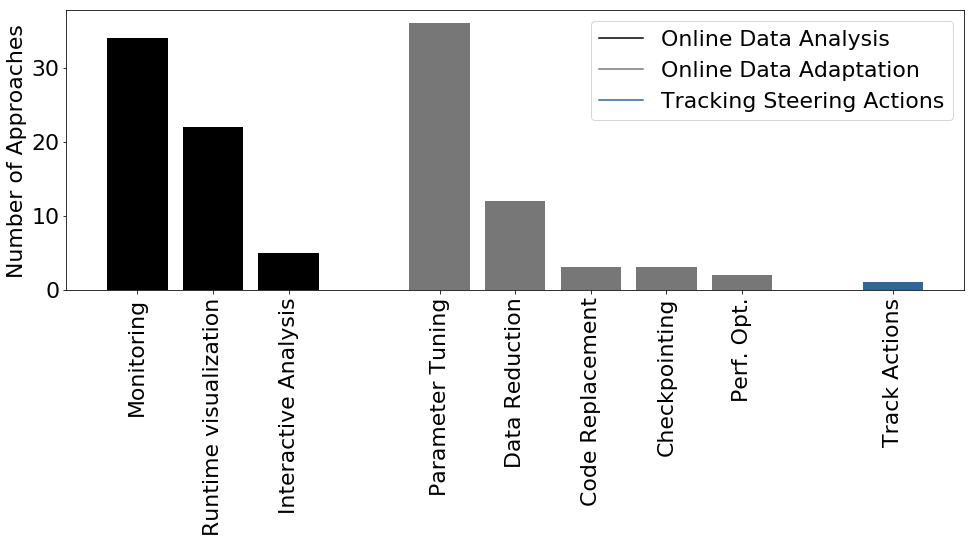
\includegraphics[width=\textwidth,keepaspectratio]{img/tab31.png}
    \caption{Summarization of Table \ref{tab:comparative_tables_systems}.}
    \label{fig:figtab31}
\end{figure}


\subsubsection{Approaches without a Workflow Management System}

GRASPARC \cite{Brodlie1993GRASPARC:}
maintains a history tree, but it is used for checkpointing and rolling
back.
Falcon \cite{Gu1995Falcon:} collects trace data and stores in a database. It also has
Trace data collector, Trace data analyzer, and a Trace data database.
These traces are used for debugging and \textit{post-hoc} analyses.
Its runtime data capture is limited, with no integration with domain
and performance data. Steering action data are not
captured. There is no support for exploratory online data analyses. There
are no explicit data relationships between the user's steering actions with
the results of a steering action. Furthermore, they show little use of
the traces database in their paper, making it harder to evaluate
the benefits of having such a database.

\citet{Danani2015Computational}'s work uses a DBMS for registering user records and
generic application data.
Despite the data analytical component in their architecture, it is not
clear if it can be used for online data analyses to facilitate knowledge
discovery in large amounts of scientific data and to relate to user
steering data. \citet{Shu2011Computational,Shu2006WBCSim:} use a DBMS to facilitate development of WBCSim.
It stores simulation input and results, thus can be used for analyses.

DfAnalyzer \cite{Silva2017Raw,Camata2018In,silva_dfanalyzer:_2018} allows for rich dataflow online analysis in large-scale workflows. It contributes by providing workflow provenance data analysis enriched with execution data and domain data through runtime data extraction and indexing techniques.
DfAnalyzer materializes dataflows by relating elements from raw data files. Through manual instrumentation of workflow script, users add lightweight library calls with negligible overhead to the workflow execution. It can be combined with ParaView Catalyst to allow for \textit{in-situ} data capture and runtime visualization. Based on data analysis provided by DfAnalyzer, CSE users were able  to steer a running workflow \cite{Camata2018In}.
However, like all the other approaches, DfAnalyzer does not manage user steering action data, thus users cannot understand how their actions are influencing a running workflow, which is a critical aspect that needs to be supported in the workflow steering lifecycle.

Therefore, none of these approaches manage steering action data, \ie{} they do not capture steering action data, relate to the workflow data, and store in a database available for analysis at runtime, which would allow users to analyze steering action data online, supporting the workflow steering lifecycle.


\subsubsection{Approaches with a Workflow Management System}

Data managed by current WMS execution engines are separate
from data for provenance and analyses. During the execution, the WMS
manages its internal scheduling data to be efficient for parallel
performance and generates logs to be structured for queries for
provenance data analyses after the execution ends. That is, execution
data are not available for online queries when a workflow is running.
There are important limitations with this approach of not making
execution data available from data analyses at runtime.

A major shortcoming is the lack of support for monitoring queries
involving domain data from data structures or repositories, which remain
isolated from execution data. This prevents a WMS from providing
support for monitoring queries like ``how many tasks are still pending to
be scheduled for the workflow activity 3?'' or ``what is the average
execution time for the tasks that have already executed?'', and debugging
queries like ``how long was the average execution time for tasks that
produced a result value greater than x?''. The problem is that the user
who models a workflow often needs to fine-tune its configuration.
Analytical queries, with performance data (\eg{} task duration,
memory or CPU consumption by task, etc.) and domain data, can show
whether the workflow is in the right direction or needs further
adjustments. When these data are separated, submitting a monitoring or
debugging query is quite complex, leading to the classic problem of data
integration for analysis \cite{Jagadish2014Big}.

Besides, if performance data are not adequately registered during
workflow execution, they will no longer be available for analyses when
the execution finishes. Another problem is the difficulty for providing
runtime data analysis since provenance is only registered in log files,
which are much harder to be queried than structured or semi-structured
data. To facilitate dealing with data management issues, WMS solutions often
make use of DBMS. In this section, we briefly discuss how DBMS take part
in existing WMS architectures and which role they play in terms of user steering capabilities.

Swift/T \cite{Wozniak2013Swift/T:,Duro2016Flexible}
is a highly scalable approach that uses a distributed key-value store to
enforce data dependencies between tasks during scheduling execution, but
it does not allow for tracking user steering action.
To keep its high scalability,
Swift/T stores analytical data in log files, which are loaded to a DBMS
only when the workflow execution finishes. Still, there are two
databases, which use different DBMS to manage them and the user does not
have access to the database used by Swift's engine for scheduling.

Pegasus \cite{Deelman2015Pegasus}
is also a scalable WMS that has been used for many real-world workflows, like LIGO for gravitational wave
discovery \cite{PhysRevLett.118.221101}.
Pegasus uses a DBMS to store execution data, which is available for the
user to do runtime execution monitoring, but does not provide for data
analyses based on runtime \emph{ad-hoc} queries. Like Swift, Pegasus
also stores provenance data in log files to be made available for
user queries only after the workflow finishes.

Stampede \cite{Gunter2011Online} is a DBMS-based
execution monitoring tool that can be plugged into WMSs. Stampede adopts
a centralized DBMS solution and has been evaluated with two different
WMSs, Pegasus and Triana, to show its monitoring facilities. However, it
is also a solution that does not integrate monitoring to domain or
provenance data, and does not allow for tracking steering actions.

FireWorks is a scalable WMS \cite{Jain2015FireWorks:}
that also has a DBMS-driven workflow execution engine. FireWorks has a
JSON-based approach to state management and uses MongoDB to support
scheduling queues and queries JSON documents to monitor workflow
execution. FireWorks's approach shows scalable results when monitoring
concurrent workflows' executions. Even though MongoDB is a distributed
document-oriented DBMS, FireWorks communicates with MongoDB as a centralized
database server, which suffers from many concurrent accesses. Also, as a document-oriented DBMS, MongoDB has limited query
capabilities for relating different workflow data and limited
\emph{ad-hoc} analytical queries.

Chiron \cite{Ogasawara2011algebraic, Dias2015Data-centric}
collects provenance data and uses a centralized, relational DBMS to
integrate and manage data required for parallel execution and data for
analytical queries. It is the only WMS that manages execution, domain, and provenance data in the same database, making it an exception among the approaches within WMSs.
SciCumulus \cite{Oliveira2010SciCumulus:} is a lightweight middle on top of Chiron that adds capabilities to exploit cloud computing environments.
d-Chiron \cite{souza_controlling_2015_thesis,Souza2015Parallel}
is a version of Chiron that employs a highly efficient in-memory distributed DBMS to accelerate the parallel execution control in Chiron. However, as the other WMSs, neither Chiron or any of its versions can manage steering action data without the concepts and techniques introduced in this thesis.


Therefore, we are not aware of any WMS approach that manages steering action data or allow the users to track their steering actions, compromising the workflow steering lifecycle support.


\subsubsection{Other Approaches for User Steering}

Other approaches \cite{Reyes2010Monitoring,Matkovic2014Visual,Cordasco2013Designing}
provide some user steering support, like parameter tuning,
reduction of parameter space, performance tuning, and monitoring.
However, they provide little or none data analytical support, no provenance data
management, and no steering action data management.

Moreover, while most approaches that enable data reduction aim at avoiding data to be generated, \eg{} by
enabling users to prune useless solutions in a large solution space,
there is an intense area of data reduction research focused on reducing
data already generated by the simulation. For example, initiatives like
CODAR \cite{Foster2017Computing},
Melissa \cite{Terraz2017Melissa:},
DimStiller \cite{Ingram2010Dimstiller:},
and the work by \citet{Jin2013Using},
propose data reduction strategies such as dimension reduction, outlier
detection and compression also based on online data analyses, which are
complementary to our approach. Other approaches provide steering support
but are too application or domain-specific, such as Computational Fluid
Dynamics \cite{Garcia2015Computational},
whereas we aim to design a domain and application-independent solution.

\citet{Spinuso2018Active} has investigated the importance of  capturing provenance data at runtime for steering in scientific workflows, in an approach called \textit{Active}. Among several contributions, he proposes S-PROV, a provenance data diagram extension of  W3C PROV, to represent workflow abstractions and concretization in the execution of real use cases.
The main difference between \textit{Active} and our approach \textit{WfSteer} is that we aim at supporting computational steering in large-scale workflows, such as the ones found in CSE applications that require large HPC machines, which adds new challenges as already discussed.
Additionally, another difference is that we addressing the challenge to enable efficient capture and query of provenance  data considering use cases both with and without WMSs, which adds a new complexity to the problem.
Therefore, we believe our detailed characterization of steering actions, along with the notion of provenance of the steering action data and our proposed W3C PROV-compliant representation of these concepts, and the design principles for efficient steering action data capture in HPC considering both with and WMSs is complimentary to the \textit{Active} approach.


Recent works \cite{Zhang2017Diagnosing,Re2015Machine,Xin2018Accelerating,souza_provenancedata_2019}
have explored user steering concepts for parameter tuning; data
capture for analysis, monitoring, and debugging; and data reduction
applied to Machine Learning life cycle (\eg{} data preprocessing,
training, models, result analyses).

Figure \ref{fig:chap1_10} \cite{Meignan2015Review}
shows a conceptual interactive optimization approach, such as human-guided
search, for Operations Research. Because an optimization model ``may
underestimate or ignore some aspects of the real problem'', resulting in
computation of either ``unrealistic or unfeasible solutions, or
solutions that do not capture domain-related characteristics'', several
contributions in Operations Research have been made to overcome this.
For example, robust optimization to deal with the inherent uncertainty
of a decision context. However, even with such improvements in
Operations Research, there are still limitations such as to find an
efficient optimization method or, regardless the optimization model
previously designed, there may be specific decision criteria that remain
unknown and will only be found during the decision-making process. For
this, interactive optimization can be used and they share the same
motivations as ours. However, most of the approaches that provide some
support for interactive optimization do not use an online approach,
requiring the simulation to stop, tune, and re-submit. Also, making
sense of very large raw datasets is not a focus.



\begin{figure}
\centering
\begin{subfigure}{.3\textwidth}
  \centering
  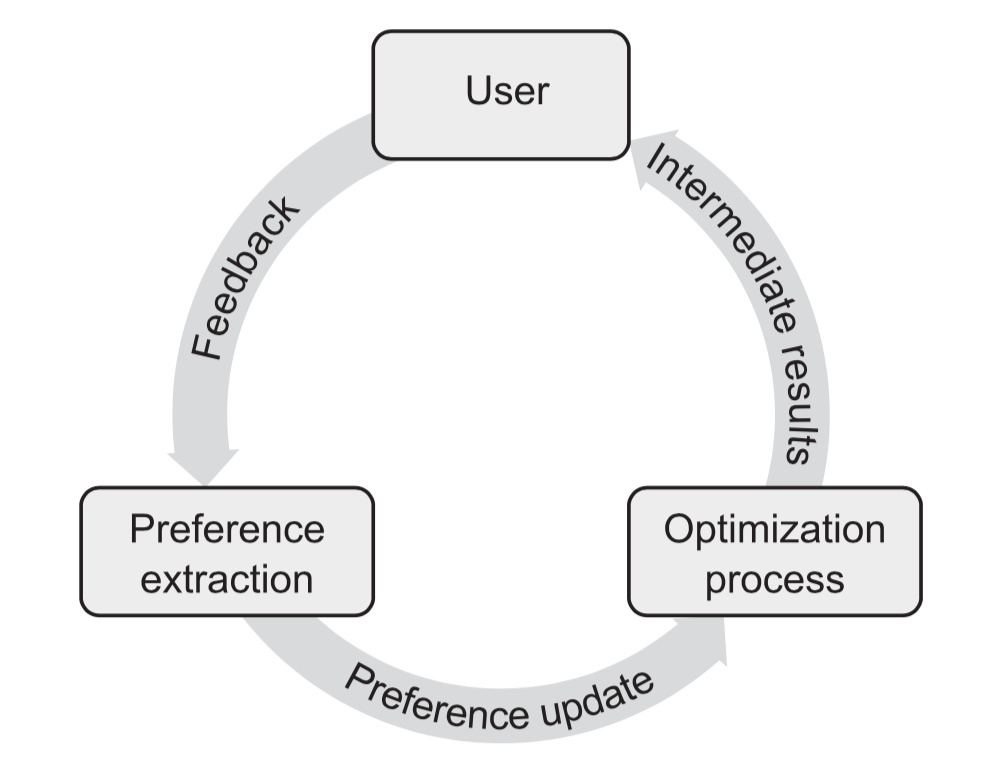
\includegraphics[width=1.0\linewidth]{img/media/image20.png}
  %\caption{A subfigure}
  \label{fig:sub1}
\end{subfigure}%
\begin{subfigure}{.7\textwidth}
  \centering
  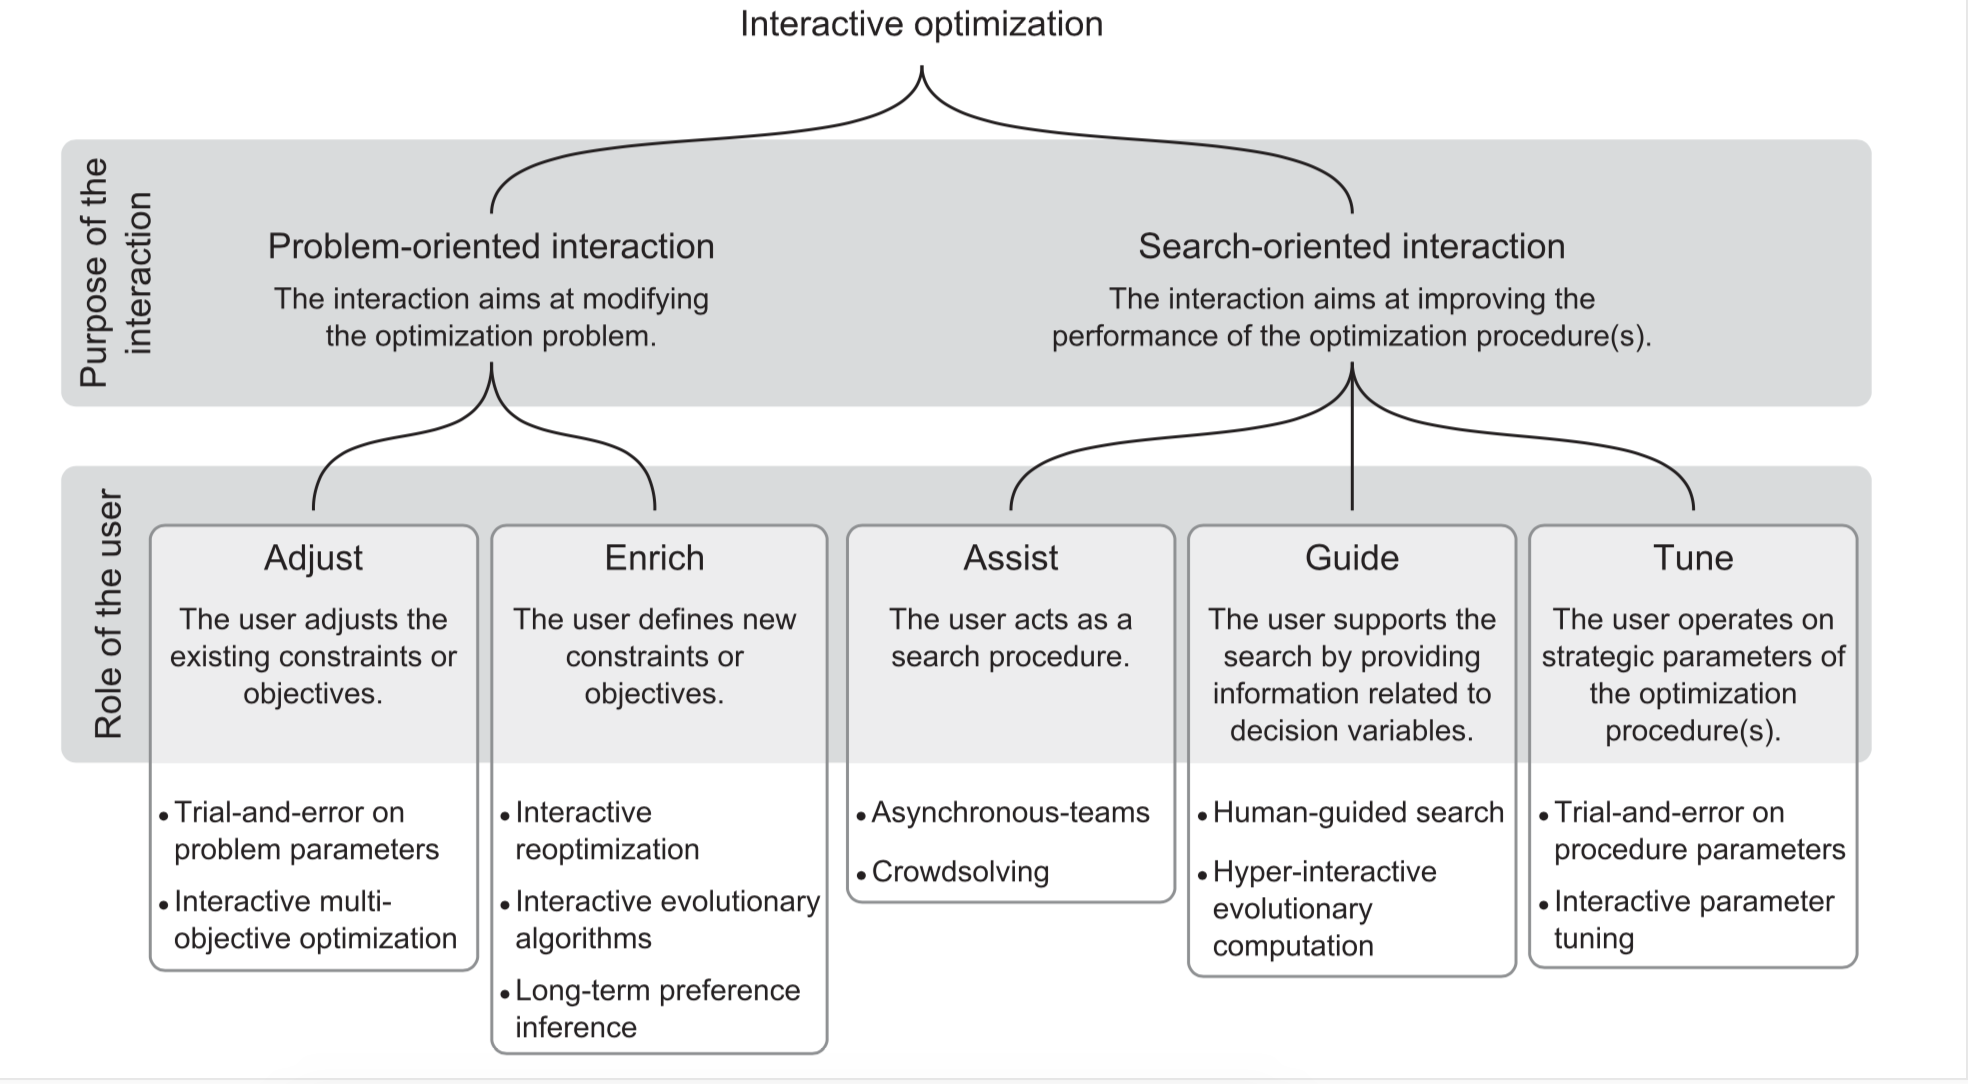
\includegraphics[width=1.0\linewidth]{img/media/image21.png}
  %\caption{A subfigure}
  \label{fig:sub2}
\end{subfigure}
\caption{User steering approach for optimization
\cite{Meignan2015Review}.}
\label{fig:chap1_10}
\end{figure}


ADIOS \cite{Lofstead2008Flexible},
GLEAN, Damaris/Viz, Qiso, Nessie, Strawman, Decaf
\cite{Dreher2017Decaf:}
enable strong monitoring and online data visualization features, but no
adaptation, nor steering action tracking. WMSs like WINGS/Pegasus
\cite{Deelman2015Pegasus},
Swfit \cite{Wozniak2013Swift/T:,Duro2016Flexible},
Nimrod/Kepler \cite{Abramson2008Nimrod/K:},
VisTrails \cite{Vistrails2014VisTrails}
have monitoring and data analyses support, but no adaptation nor steering action tracking. In the next section, we analyze these WMSs in detail regarding their data analysis and provenance management support.



\section{Making a CSE Application Steerable}

In Table \ref{tab:making_cse_steerable}, we summarize how each analyzed approach makes a CSE application steerable and Figure \ref{fig:figtab3.2} shows the amounts of approach per category.
Here, we want to analyze how they expose the data to be steered by the user. For instance, if they use message passing-based or
data-oriented implementation for communication between the running
parallel application and the user who is steering. The importance of this in the context of this thesis is that to be able to capture steering action data, our solution needs to be aware of how the CSE application is made steerable.


\begin{longtable}
{ 
 M{.17\textwidth}||
 M{.75\textwidth}
}
\caption{Comparison of implementation on how the approaches make a CSE application steerable.}
\label{tab:making_cse_steerable}\\
\hline
\hline
\hline
\hline
 \rowcolor{TableHeaderColor}

  \textbf{Approach} &
  \textbf{How the approach implements steering in a CSE application}
  \\
 \hline
 \hline
 \hline
 \endhead
 
\textbf{DfAnalyzer}
\cite{Silva2017Raw,Camata2018In,silva_dfanalyzer:_2018}
 &
Manual source code instrumentation. Communication between the user application and the backend is done via HTTP RESTful API calls.
\\
\hline

\textbf{VASE} \cite{Jablonowski1993VASE:}
&
Manual source code instrumentation.
Addition of steerable points in the data
dependencies of a dataflow. Communication between the user application and the backend is done via simple file-based communication.
\\
\hline


\textbf{SCIRun}  \cite{Parker1995SCIRun:}
&
User has to write  a C++ abstract program using the system's structure
\\
\hline


\textbf{CSE} \cite{Liere1996Computational,Liere1997Computational,Wijk1994Environment}
&
User needs to write ``satellites" and plug to their application to communicate with the ``Data Manager"
\\
\hline

\textbf{Progress and Magellan} \cite{Vetter1999Techniques}
&
Via manual source code instrumentation, user specifies only relevant data structures (called ``steering object model") to be exposed for steering. The server executes as a separate thread in the same memory space of the application.
\\
\hline


\textbf{CUMULVS} \cite{Kohl2006Cumulvs:}
&
Manual source code instrumentation to indicate data dependencies and steerable parameters.
\\
\hline

\textbf{VIPER}  \cite{Rathmayer1997tool}
&
Manual source code instrumentation.
\\
\hline

\textbf{MOSS} \cite{Eisenhauer1998Object-based}
&
Moss provides high-level  abstractions  for manual source code instrumentation of steerable  data structures and parameters. It provides performance and consistency control studies.
\\
\hline

\textbf{gViz} \cite{Wood2003gViz}
&
Manual source code instrumentation via a steering library.
\\
\hline

\textbf{DISCOVER} \cite{Mann2001DISCOVER:}
&
Manual source code instrumentation. It supports geographically distributed users steering. It uses MPI for data collectors and adaptors between the running code and the steering server. Uses Java RMI between the server and the UI.
\\
\hline

\textbf{MoSt} \cite{Glasner2001Monitoring}
&
It allows for dynamic source code instrumentation.
\\
\hline



\textbf{GRASPARC} \cite{Brodlie1993GRASPARC:}
&
Manual source code instrumentation.
\\
\hline

\textbf{ParaView Catalyst Live} \cite{Ayachit2015ParaView,Bauer2016In}
&
Manual source code instrumentation. In time-loop simulations, the simulation data structures are re-mapped at each time step in a time-loop.
\\
\hline



\textbf{PathFinder}
 \cite{Reed1996Next}
&
Manual source code instrumentation.
\\
\hline


\textbf{Extempore} \cite{Swift2015Live}
&
Users need to use a specific programming language.
Just-in-Time compilation. ``Hot-swapping" or ``live programming" of a main loop.
\\
\hline


\textbf{Cactus} \cite{Goodale2003Cactus}
&
Manual source code instrumentation.
\\
\hline


\textbf{EPSN} \cite{Esnard2006Steering}
&
Manual source code instrumentation.
\\
\hline


\textbf{pV3} \cite{Haimes1996Concurrent}
&
Manual source code instrumentation of a main loop code. It uses API to communicate with the backend.
\\
\hline


\textbf{RealityGrid} \cite{Pickles2005practical}
&
APIs for manual source code instrumentation. It addresses consistency issues. File-based and Socket-based between running application and server. SOAP for messages between client and server.
\\
\hline


\textbf{EPIC} \cite{Kress2016Visualization}
&
Manual source code instrumentation.
\\
\hline


\textbf{CS\_Lite}  \cite{Figueira2004CS_LITE:}
&
Manual source code instrumentation. It uses socket-based communication between the user application and the backend.
\\
\hline


\textbf{I-WAY} \cite{Parashar2005Grid}
&
Manual source code instrumentation.
\\
\hline


\textbf{Falcon} \cite{Gu1995Falcon:}
&
Manual source code instrumentation. It is concerned with performance, can control overheads, turn on and off each steering point, selective monitoring
\\
\hline


\textbf{Autopilot} \cite{Ribler1998Autopilot:}
&
Manual source code instrumentation. It is toolkit with data collectors and adaptors.
\\
\hline


\textbf{WBCSim}  \cite{Goel1999WBCSim:,Shu2011Computational,Shu2006WBCSim:}
&
Manual source code instrumentation.
\\
\hline


\textbf{\citet{Yi2014In-situ}}
&
File-based implementation.
\\
\hline


\textbf{\citet{Ma2007In-situ}}
&
File-based data communication.
\\
\hline


\textbf{\citet{Han2016Hybrid}}
&
Manual source code instrumentation.
\\
\hline

\textbf{\citet{Matkovic2011Adaptive}}
 &
Users need to develop inside a monolithic system
\\
\hline


\textbf{\citet{Butnaru2013Computational}}
&
Both non-intrusive and source code instrumentation are provided.
\\
\hline


\textbf{\citet{Knezevic2011Interactive}}
&
Manual source code instrumentation of CSE applications. MPI-based between user steering and the running application. Examples in CFD use cases. \\
\hline


\textbf{\citet{Danani2015Computational}}
&
Modification of RealityGrid source code to use the UI inside a HPC machine network. Useful for HPC machines that do not accept external connections, like Blue Gene/Q (the one they used) and Lobo Carneiro.
\\
\hline
 
%%%%%%%%%%%%%%%%%%%% BEGIN WMS 
\textbf{Chiron WMS}
\cite{Dias2015Data-centric,Goncalves2013Performance,Santos2013Runtime}
&
Dataflow-oriented WMS. Non-intrusive. As any WMS, it can conflict with applications that already are parallel.
\\
\hline

\textbf{WorkWays}
(on top of Nimrod/Kepler WMS)
\cite{Nguyen2015WorkWays:}
&
Science Gateway. Non-intrusive. As any WMS, it can conflict with applications that already are parallel.
\\
\hline


\textbf{gridMon Steer} (on top of Triana WMS) \cite{Wang2006gridMonSteer:}
&
Non-intrusive. As any WMS, it can conflict with applications that already are parallel.
\\
\hline
%%%%%%%%%%%%%%%%%%%% END WMS 



\hline
\hline
\hline

\end{longtable}



\begin{figure}[H]
    \centering
    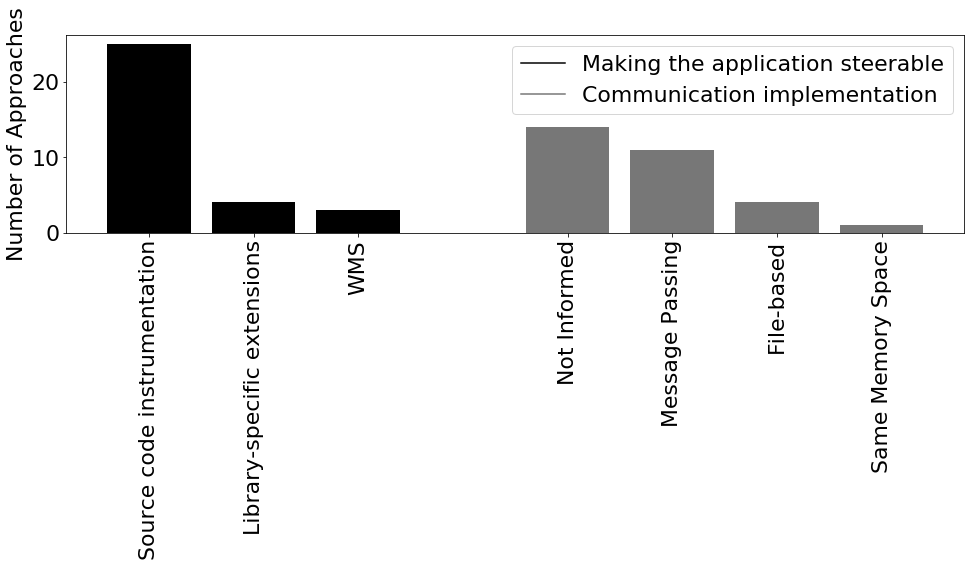
\includegraphics[width=\textwidth,keepaspectratio]{img/tab32.png}
    \caption{Summarization of Table \ref{tab:making_cse_steerable}.}
    \label{fig:figtab3.2}
\end{figure}


Users can develop their own \textit{ad-hoc} way to implement
an adaptable application, such as using a simple file-based approach
\cite{Camata2018In}.
Such implementations are usually lightweight but unsuitable for reuse,
as argued by \citet{Bauer2016In}.
General-purpose systems or frameworks or libraries that provide
user Steering support are more suitable for a universal reuse
\cite{Bauer2016In}.
We investigate how such approaches can modify a running code.
Approaches that ease data parallelism control, like WMSs with steering support
\cite{Dias2015Data-centric,Nguyen2014WorkWays:,Souza2017Data},
provide non-intrusive strategies to support parameter sweep workflows, but cannot support applications that run as workflow scripts, like the ones we describe in Section \ref{subsec_scripts}.
Other approaches and libraries enable
users to manually instrument their source code for external invocations
to a steering library \cite{Ayachit2016Performance,Bauer2016In,MulderSurvey}.
Although ``manually'' may be an issue, in a way that there are solutions that aim to enable autonomous ways to instrument a source code
\cite{Pimentel2017noWorkflow:},
manual instrumentation is a typical routine in the daily life of CSE
application developers \cite{Bauer2016In,Silva2018Capturing}.
Users that develop such applications are used to writing external calls
to parallel libraries in their application source code. They know very
well where to add such calls in their code so they know which aspects
should be steered during execution. Manual instrumentation allows users
to customize the solution to their specialized needs, as argued by \citet{Gu1995Falcon:},
who developed steering support in Falcon.


Solutions that provide autonomous code instrumentation to
capture data at runtime may pollute the source code and the online data
analysis as they may collect more data than the data that are actual
relevant for the users, and they can add unnecessary overheads by
collecting data that the user will likely never use
\cite{Silva2018Capturing,Stamatogiannakis2016Trade-Offs}.
These approaches that support steering by allowing the user
to manually instrument their application in strategic ``steerable''
points of their application code are suitable for CSE applications,
which is a limitation for the WMSs that support steering. However, if
the added code for instrumentation is overwhelmingly complex for the
user, too many lines need to be added, or significant performance
overheads are added, this may be a problem for adoption of the solution,
as discussed by the authors of CS\_Lite
\cite{Figueira2004CS_LITE:}.



\section{System Design of an Approach that Supports User Steering}

By surveying these approaches, we identify two main strategies to implement steering: data-oriented or message
passing. In the data-oriented strategy, there is a shared data space
between the running parallel application and the system supporting
steering. The majority of these approaches using the data-oriented strategy
adopt a file-based implementation, \ie{} files in the file system
are the ``shared data space''. The file is accessible both by the user
steering the running application and by the application itself. If the
user changes the file, the application reloads its settings based on the
new values in the file. The advantages of this implementation are that
it is very simple and lightweight, and it does not require extra
software or libraries \cite{Pickles2005practical}.
However, if there are multiple checks in this file in a very short
time, or if there are multiple modifications at once, or if a
high performance shared disk (\eg{} Lustre, GPFS) is not
available, this may impact the overall performance of the simulation. In
addition to performance, another issue that may arise is consistency. If
a user modifies an application while it is running, how to guarantee
that the adaptation will not cause an error or lead to an inconsistent
state? For instance, during execution often there are thousands of tasks
to run in parallel. Some of them are already running, others have
already executed, and others are waiting to be executed. If the user
tries to steer the execution affecting an already executed task, the
steering action may not take effect; or if the user tries to modify a
task that is executing, like performing calculations or writing data
files on disk, this may lead the execution and data (\eg{}
overwriting files that were being written) to an inconsistent state.
Moreover, when designing a steerable application, one needs to be
concerned with a ``steering lag'' \cite{Hart1999Consistency},
which is the elapsed time between the user interaction and the steering
action to take place in the running parallel application.

In addition to data-oriented, other implementations use a client-server
architecture, via \myabbrev{MPI}{Message Passing Interface}, sockets or \myabbrev{HTTP}{HyperText Transfer Protocol} for message passing between the
user interface, the running application, and the system providing
steering support. We explain which implementation each approach uses in
Table \ref{tab:making_cse_steerable}. In these implementations, there are no disk accesses for
steering, which may be a better strategy for \emph{in-situ} steering.
However, we found no performance and consistency issues being further
addressed in those works. As mentioned by
\citet{Ayachit2016Performance},
there was no focused effort to study the scalability of these approaches
nor the overhead they add to parallel workflow script (\ie{} the simulation code).
Besides, some approaches \cite{Vetter1999Techniques,Xian2008Computational}
use the terms ``sensors'' and ``actuators'' to signify runtime relevant
data capturers and adapters of steerable data.



\section{Further Discussion on the Analyzed Approaches}

We analyzed several approaches and their support for steering. The publications of three of them, RealtyGrid \cite{Pickles2005practical},
Magellan \cite{Vetter1999Techniques},
and Mulder's \cite{MulderSurvey},
contain high-level illustrations (Figures \ref{fig:fig3_1}, \ref{fig:fig3_2}, and \ref{fig:fig3_4}, respectively) of an approach
that provides traditional user steering support.
In common, they have three main
components: the user interface (from where users analyze and steer the
parallel application); the system that supports steering; and the
parallel application that is going to be steered by the user.

\begin{figure}[H]
    \centering
    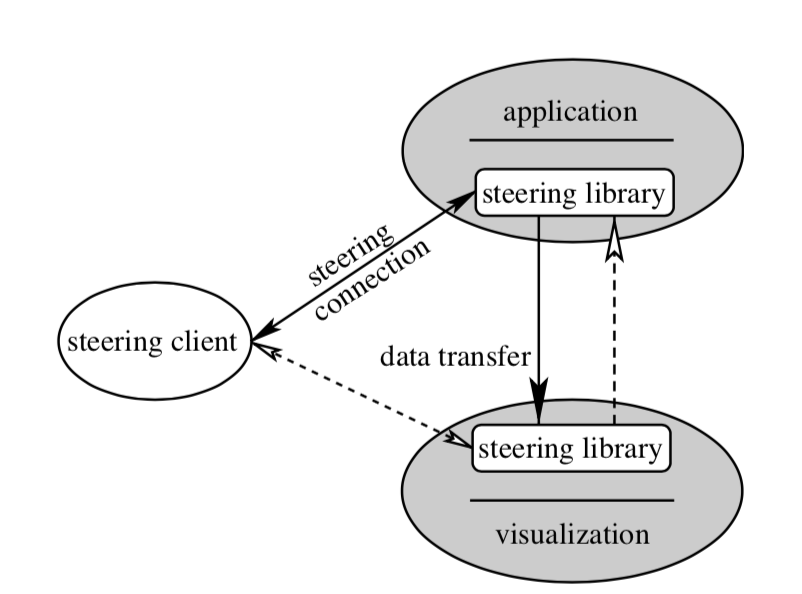
\includegraphics[width=300px,keepaspectratio]{img/media/image11.png}
    \caption{Basic components of an approach that supports user steering, according to \citet{Pickles2005practical}.}
    \label{fig:fig3_1}
\end{figure}

\begin{figure}[H]
    \centering
    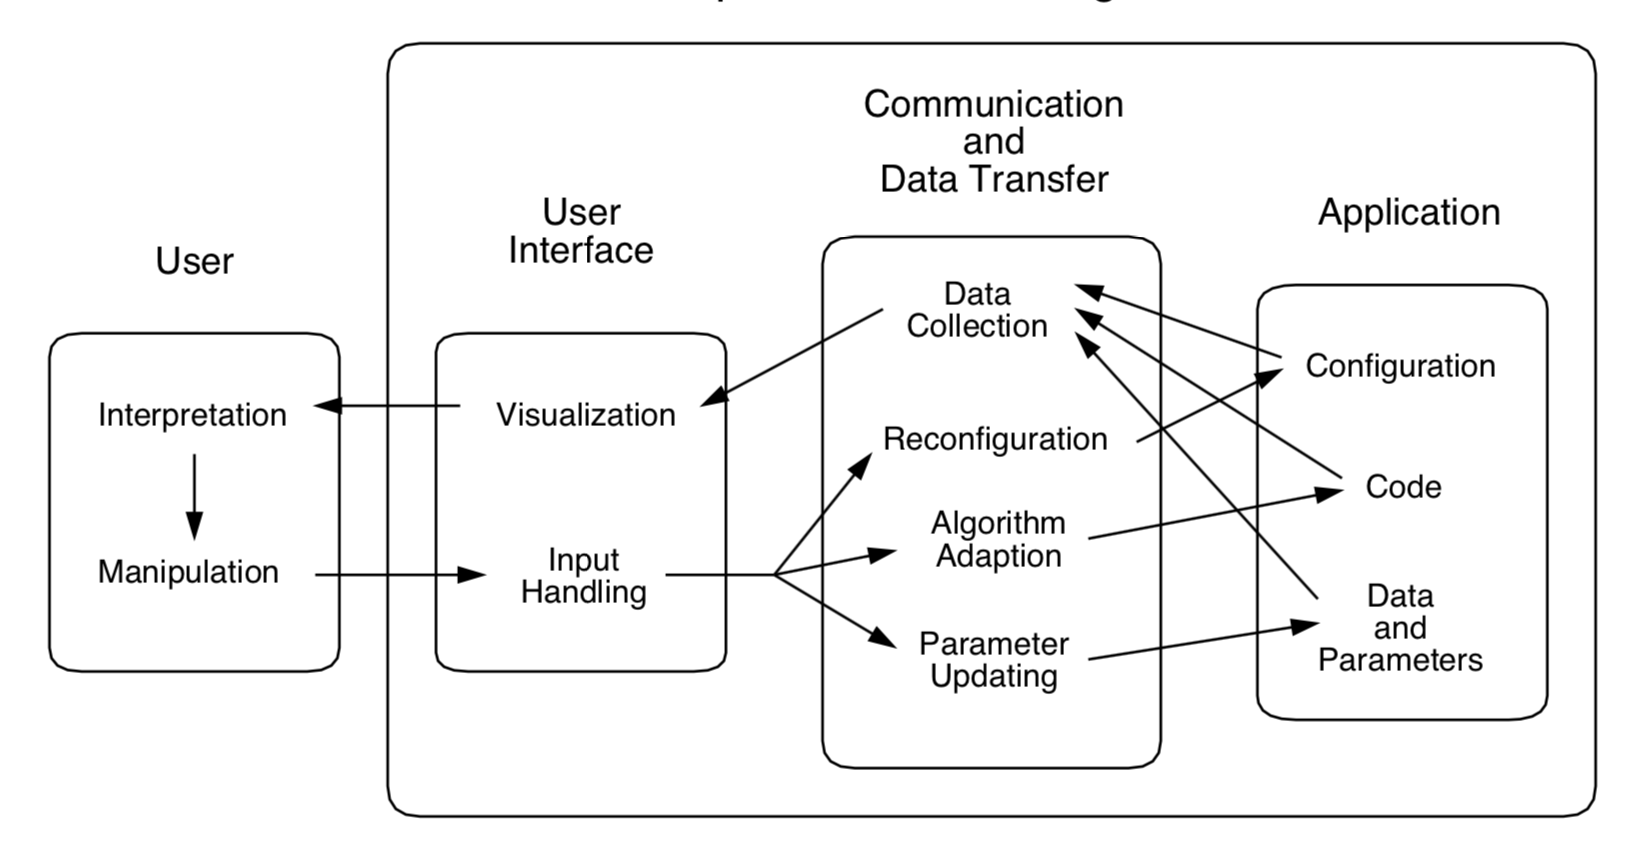
\includegraphics[width=400px,keepaspectratio]{img/media/image12.png}
    \caption{User steering concepts, according to
\citet{MulderSurvey}.}
    \label{fig:fig3_2}
\end{figure}

\begin{figure}[H]
    \centering
    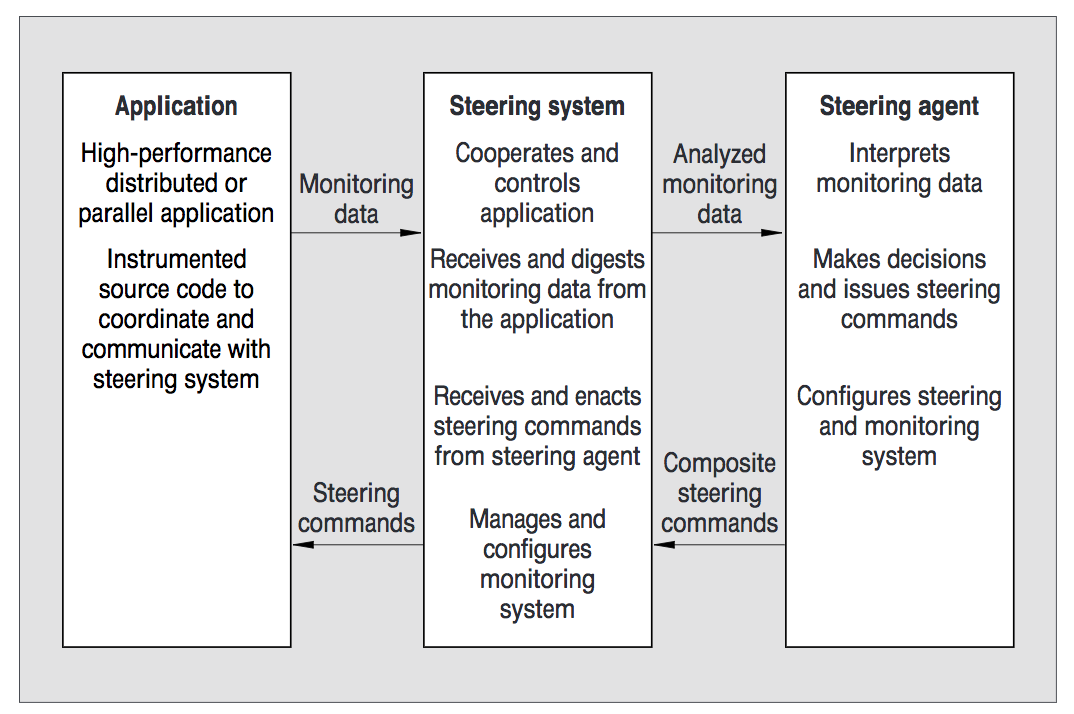
\includegraphics[width=400px,keepaspectratio]{img/media/image14.png}
    \caption{Conceptual view of a approach that supports steering according to \citet{MulderSurvey}.}
    \label{fig:fig3_4}
\end{figure}



\noindent Figure \ref{fig:fig3_3} shows a general architecture for
interactive optimization, which considers human feedback for building a
preference model to help users to steer
\cite{Meignan2015Review}.

\begin{figure}[H]
    \centering
    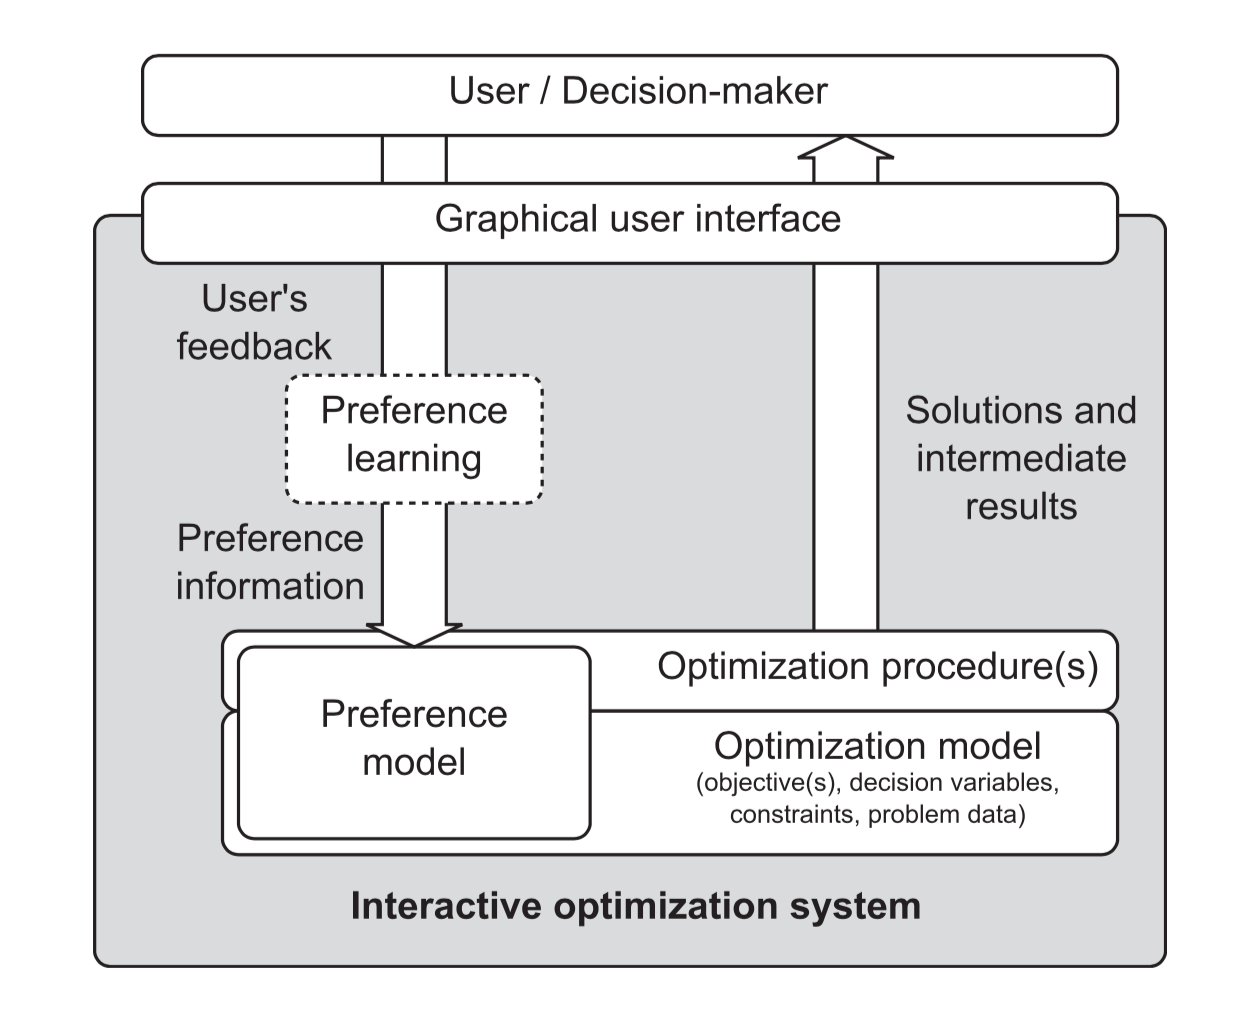
\includegraphics[width=300px,keepaspectratio]{img/media/image13.png}
    \caption{User steering for Operations Research
\cite{Meignan2015Review}.}
    \label{fig:fig3_3}
\end{figure}


In Figure \ref{fig:fig3_1} \cite{Pickles2005practical},
we also see that they provide a library to be used as external calls in the
running code for visualization and steering. According to \citet{Danani2015Computational}, who deployed RealityGrid in Blue Gene/Q HPC machine,
RealityGrid has a client-side that runs on the user's desktop whereas
the server runs on the same machine that the parallel simulation runs.
This is a limitation for Blue Gene/Q and several other HPC machines,
like Lobo Carneiro\footnote{http://www.nacad.ufrj.br/recursos/sgiicex},
which disallows connections form external networks for security reasons.
Thus, they modified RealityGrid's open source code
\cite{RealityGrid},
in the client component, to run it on Blue Gene/Q. Then, they were able
to run RealityGrid in OpenFOAM, a highly parallel CFD toolbox that
contains numerical solvers. They were able to control two
parameters using RealityGrid: \emph{deltaT} and \emph{nCorr}, which are
used in the inner loop of the solver. They provide a general
architecture (Figure \ref{fig:fig3_9}) for computational steering and data analyses
for large volumes of raw data, which they call ``Future of Steering
Workflows''.

\begin{figure}[H]
    \centering
    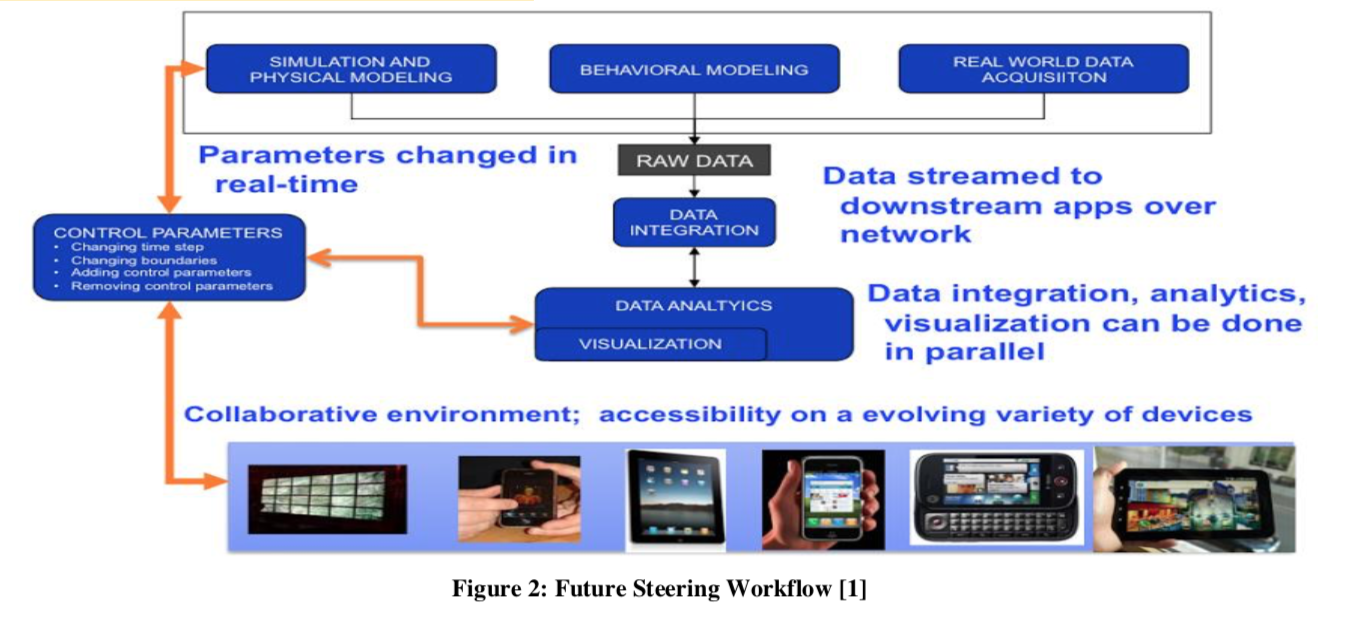
\includegraphics[width=420px,trim={0 1cm 0 0},clip,keepaspectratio]{img/media/image18.png}
    \caption{\citet{Danani2015Computational}' view on ``the future of steering workflows''.}
    \label{fig:fig3_9}
\end{figure}


Figure \ref{fig:fig3_5}, extracted from \citet{Han2016Hybrid}'s work,
shows a dynamic data-driven architecture for steering. There is a
Calibrator component that is controlled by humans and can change the
parameters and variables at runtime of a legacy source code previously
instrumented manually. Data are captured at runtime for Machine
Learning-based prediction and monitoring. They use a DBMS to store data
for the Machine Learning models. Based on analysis of the Predictor and
Monitoring, users can steer. HAN and BROOKE
are co-authors of another application
\cite{Han2014Virtual}
that runs on Blue Gene/Q. This application has a similar architecture to
the one that uses RealityGrid, which we previously discussed. This
application demonstrates an interesting modern use of this Computational
Steering: users using a mobile device, such as a smartphone, to steer a
CFD simulation running on the IBM Blue Gene/Q HPC machine.

\begin{figure}[H]
    \centering
    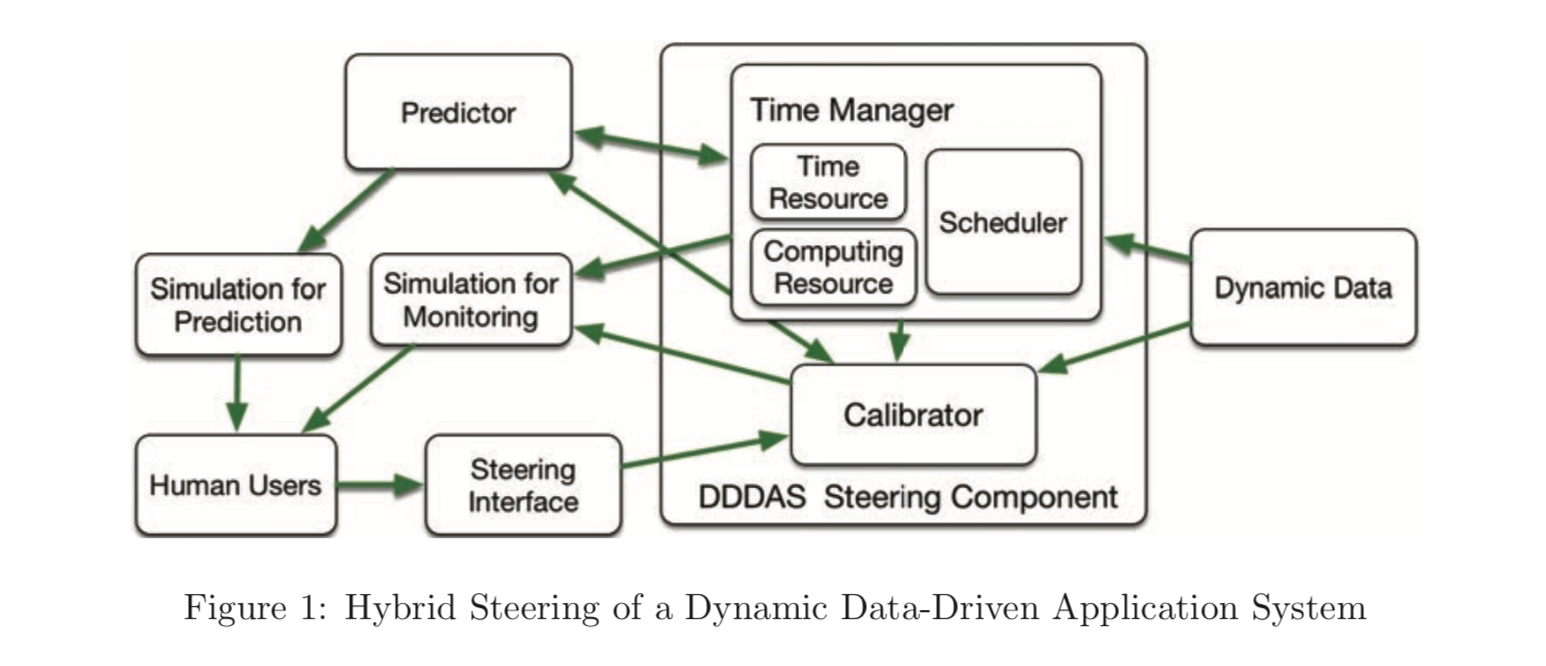
\includegraphics[width=400px,trim={0 1.3cm 0 0},clip,keepaspectratio]{img/media/image15.png}
    \caption{Dynamic data-driven steering architecture \cite{Han2016Hybrid}.}
    \label{fig:fig3_5}
\end{figure}

Another classic approach that supports steering is the so-called
``Computational Steering Environment'', developed in the nineties
\cite{Liere1996Computational,VanLiere1997Computational,Wijk1994Environment},
whose architecture is shown in Figure \ref{fig:fig3_6}. It is one of the first approaches
with user steering support. It also relies on the idea of
manual application source code instrumentation. It uses a data-driven
approach for steering. ``Satellites'' are interfaces between the user
and the Data Manager. Satellites can read and write variables (scalars
or arrays) from a database managed by a Data Manager component. When a
variable is changed as a result of a satellite command, the Data Manager
sends back a notification to confirm the change. The database managed by
the Data Manager is stored as files on disk. In this way, users of
parallel applications develop their mechanisms for reading/writing
variables to this file.


\begin{figure}[H]
    \centering
    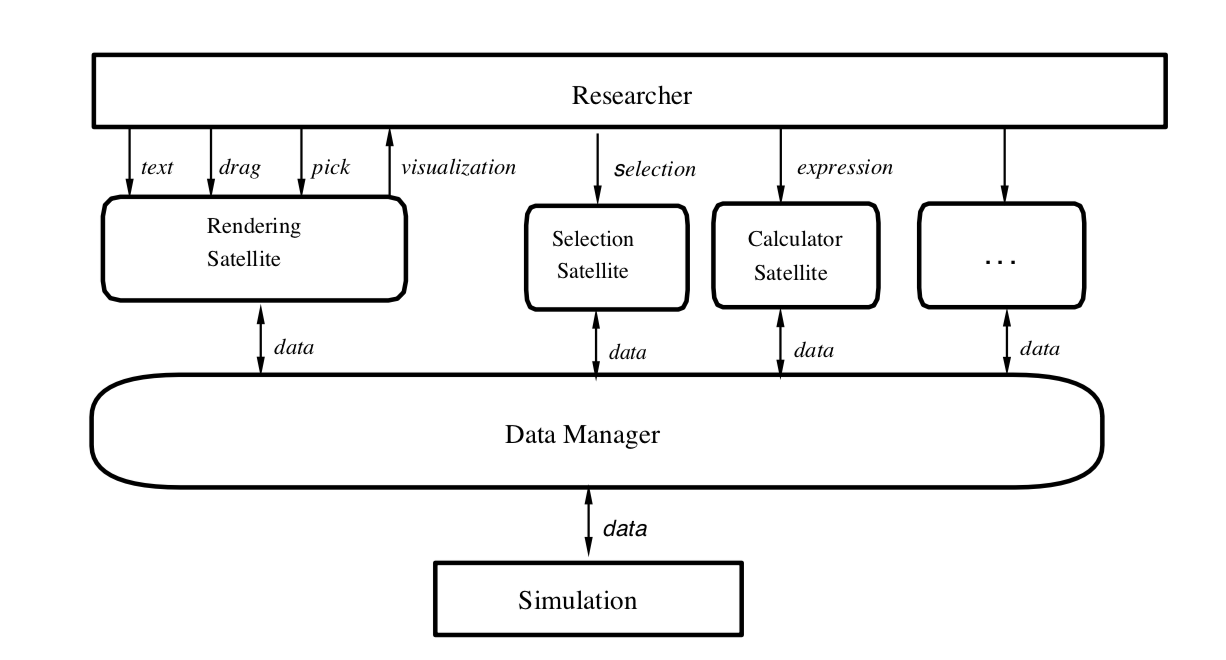
\includegraphics[width=400px,keepaspectratio]{img/media/image16.png}
    \caption{``Computational Steering Environment'' system architecture
\cite{Liere1996Computational,VanLiere1997Computational,Wijk1994Environment}.}
    \label{fig:fig3_6}
\end{figure}



Falcon \cite{Gu1995Falcon:}
is a lightweight toolkit that supports monitoring and steering. Its architecture is shown in Figure \ref{fig:fig3_7}. It has
runtime libraries for information capture, collection, filtering, and
analysis, and a graphical user interface. In Falcon, the application
code is instrumented. The user specifies monitoring to expose relevant
simulation parameters to be monitored and steered. Falcon also captures
performance data. Partially processed monitoring information is used by
the user to help to decide on what to steer. One of the main
functionalities in Falcon is to allow users to control at runtime any
added functionality to the user's running application. Users can
dynamically turn on and off any runtime data capture or steering
capabilities previously added during source code instrumentation.

\begin{figure}[H]
    \centering
    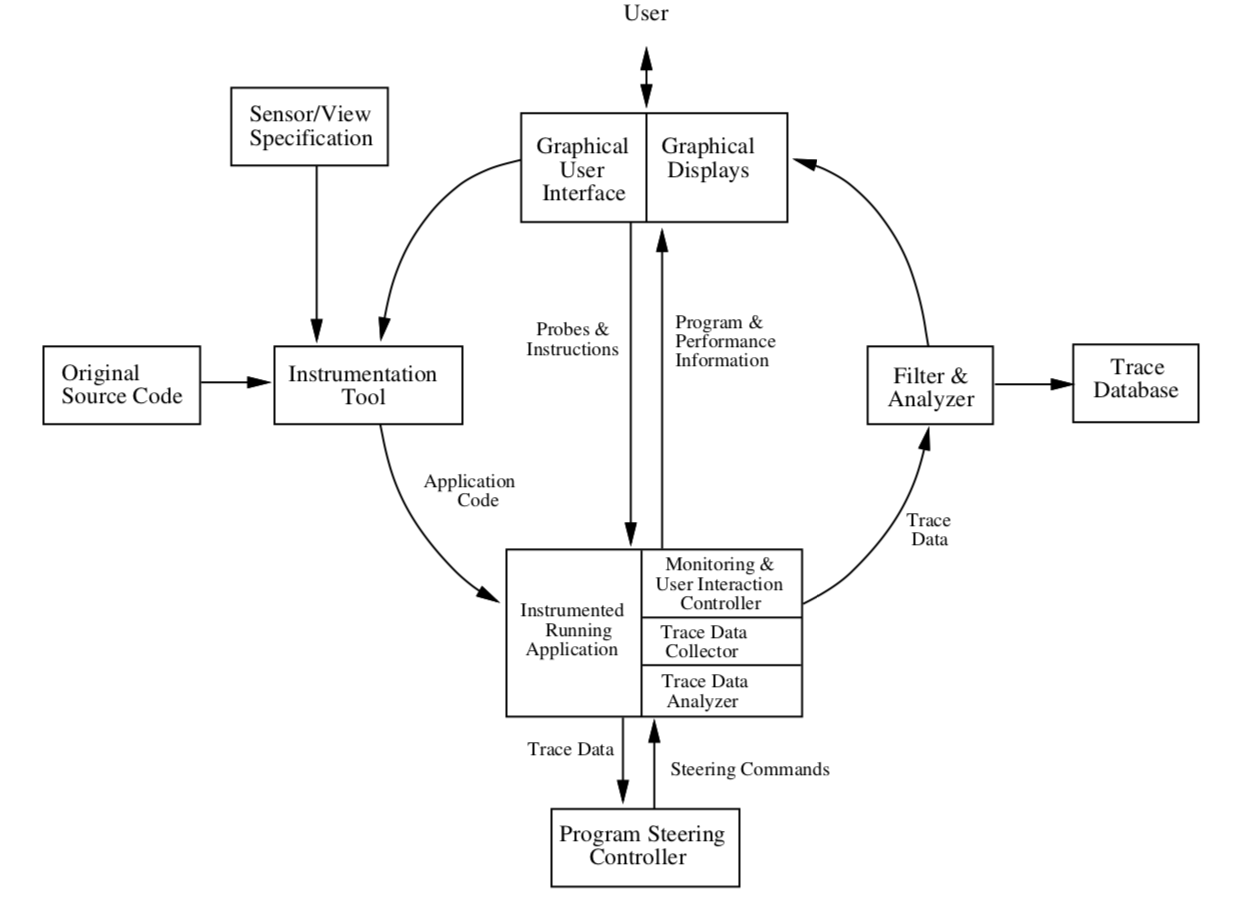
\includegraphics[width=420px,keepaspectratio]{img/media/image17.png}
    \caption{Falcon's architecture \cite{Gu1995Falcon:}.}
    \label{fig:fig3_7}
\end{figure}


WBCSim (Figure \ref{fig:fig3_8}) has been developed since 1999
\cite{Goel1999WBCSim:}.
It is another approach that supports user steering in legacy
workflow script codes. It provides a lightweight library for source code
instrumentation. It has a monitor that alerts users when it is time to
steer. It has a data visualization of simulation results. Analyzing the
behavior of the execution after a steering action, the addition of multiple
steering points, and the addition of support of a database in an idea that
is similar to the track of steering action data to compare steering
results to other results are pointed as future work
\cite{Shu2011Computational}.
Despite the important contributions for general concepts of
user steering, WBCSim's papers
\cite{Goel1999WBCSim:,Shu2011Computational,Shu2006WBCSim:}
promote deeper specialized discussions on how to support wood science
and legacy FORTRAN application codes instead of a wider variety of
scientific domains. Moreover, one of its design goals is to provide
user steering for small-scale Problem Solving
Environments, which differs from our motivations as we aim at
large-scale parallel applications.

\begin{figure}[H]
    \centering
    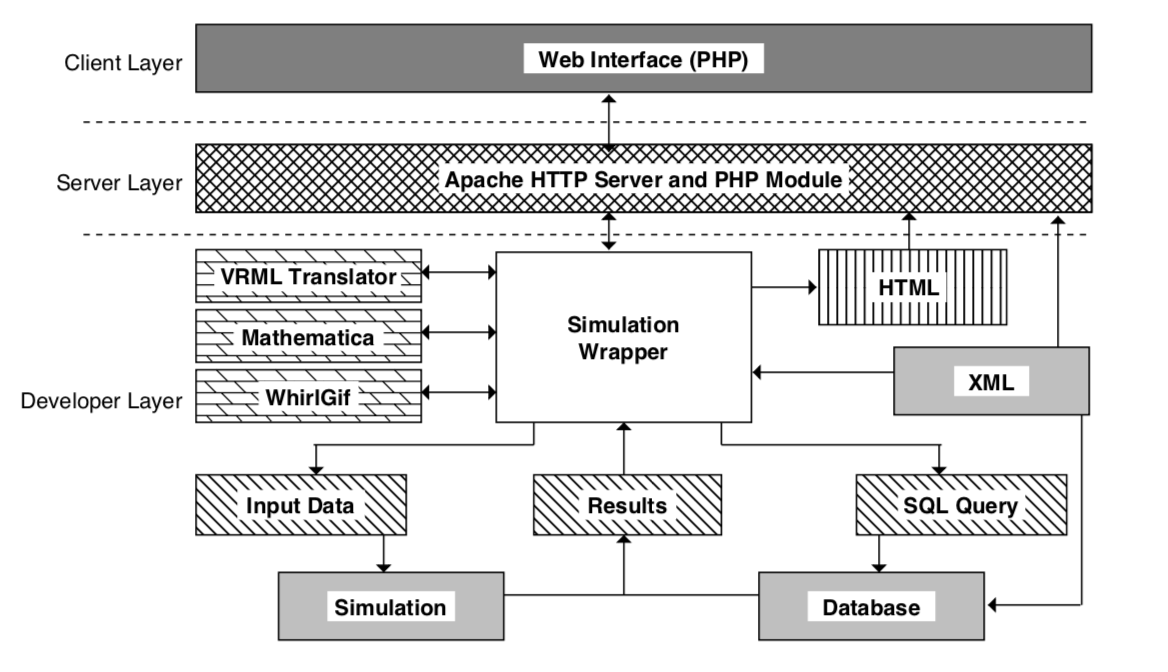
\includegraphics[width=420px,keepaspectratio]{img/media/image19.png}
    \caption{WBCSim approach architecture
\cite{Goel1999WBCSim:,Shu2011Computational,Shu2006WBCSim:}.}
    \label{fig:fig3_8}
\end{figure}

VIPER (VIsualization of Parallel numerical simulation algorithms for
Extended Research) \cite{Rathmayer1997tool}
is mainly designed for parameter space exploration. Users annotate the
program to identify data and input parameters as steerable objects. When
a steerable object is found in the code at runtime, VIPER server is
notified. It extracts data from the application or restores input
parameters. They test steering in a parallel CFD application.

MoSt (The Monitoring and Steering Environment)
\cite{Glasner2001Monitoring}
provides powerful data visualization and enables users to adapt the
running code. It also allows for steering performance optimization. One
interesting feature is its ability to instrument a running application.
This allows dynamicity even without pre-defined code instrumentation.

Extempore \cite{Swift2015Live}
is a live-programming environment. Users add calls to Extempore in their
main simulation loop. Then the loop is controlled by Extempore.
Thereafter, the user can interactively send statements to the Extempore
compiler. They are ``just-in-time'' compiled (C, C++, Fortran) into
native machine code, including MPI, and immediately executed.

ParaView Catalyst Live \cite{Ayachit2015ParaView}
is designed to run synchronously with the simulation. There is MPI
communication between simulation and analysis and it is the application
developer's responsibility to write an additional communication routine
during code instrumentation. It has efficient \textit{in-situ} data
visualization capabilities as analysis and simulation run alongside, in
the same address space. ParaView Catalyst Live enables monitoring and
steering the simulation workflow. The simulation data structures are
re-mapped at each time step \cite{Bauer2016In}.

Therefore, as surveyed by \citet{Bauer2016In}, many of these approaches are no
longer maintained.
As discussed by \citet{Figueira2004CS_LITE:}, some of them are very hard to be used,
as there are several lines of code that need to be added in the user's
application code.
\citet{Hart1999Consistency}
mention that consistency in modifying a running parallel code needs to
be considered by the steering systems developers, but we found that most
of these approaches do not address consistency problems, as mentioned in
Table \ref{tab:making_cse_steerable}.
Thus, although many approaches provide steering support and some
of them were proposed over twenty years ago, there are issues such as performance, consistency, and enabling multiple
steering actions that are not yet addressed.
Furthermore, none of these approaches allows for tracking steering actions, compromising the workflow steering lifecycle support. Except for DfAnalyzer and the WMS approaches, provenance data management techniques, which could be a solution for this, are not mentioned at all in the publications describing the approaches surveyed in this chapter.
In the next chapter, we present our approach for tracking steering actions in workflows.
